%%%%%%%%%%%%%%%%%%%%%%%%%%%%%%%%%%%%%%%%%
% Masters/Doctoral Thesis 
% LaTeX Template
% Version 2.3 (25/3/16)
%
% This template has been downloaded from:
% http://www.LaTeXTemplates.com
%
% Version 2.x major modifications by:
% Vel (vel@latextemplates.com)
%
% This template is based on a template by:
% Steve Gunn (http://users.ecs.soton.ac.uk/srg/softwaretools/document/templates/)
% Sunil Patel (http://www.sunilpatel.co.uk/thesis-template/)
%
% Template license:
% CC BY-NC-SA 3.0 (http://creativecommons.org/licenses/by-nc-sa/3.0/)
%
%%%%%%%%%%%%%%%%%%%%%%%%%%%%%%%%%%%%%%%%%

%----------------------------------------------------------------------------------------
%	PACKAGES AND OTHER DOCUMENT CONFIGURATIONS
%----------------------------------------------------------------------------------------

\documentclass[
11pt, % The default document font size, options: 10pt, 11pt, 12pt
%oneside, % Two side (alternating margins) for binding by default, uncomment to switch to one side
%chapterinoneline,% Have the chapter title next to the number in one single line
english, % ngerman for German
singlespacing, % Single line spacing, alternatives: onehalfspacing or doublespacing
%draft, % Uncomment to enable draft mode (no pictures, no links, overfull hboxes indicated)
%nolistspacing, % If the document is onehalfspacing or doublespacing, uncomment this to set spacing in lists to single
%liststotoc, % Uncomment to add the list of figures/tables/etc to the table of contents
%toctotoc, % Uncomment to add the main table of contents to the table of contents
%parskip, % Uncomment to add space between paragraphs
%nohyperref, % Uncomment to not load the hyperref package
headsepline, % Uncomment to get a line under the header
]{MastersDoctoralThesis} % The class file specifying the document structure

\usepackage[utf8]{inputenc} % Required for inputting international characters
\usepackage[T1]{fontenc} % Output font encoding for international characters

\usepackage{palatino} % Use the Palatino font by default

\usepackage[backend=bibtex,style=authoryear,natbib=true]{biblatex} % Use the bibtex backend with the authoryear citation style (which resembles APA)

\addbibresource{example.bib} % The filename of the bibliography

\usepackage[autostyle=true]{csquotes} % Required to generate language-dependent quotes in the bibliography

\usepackage{amsmath}
%----------------------------------------------------------------------------------------
%	MARGIN SETTINGS
%----------------------------------------------------------------------------------------

\geometry{
	paper=a4paper, % Change to letterpaper for US letter
	inner=2.5cm, % Inner margin
	outer=3.8cm, % Outer margin
	bindingoffset=2cm, % Binding offset
	top=1.5cm, % Top margin
	bottom=1.5cm, % Bottom margin
	%showframe,% show how the type block is set on the page
}

%----------------------------------------------------------------------------------------
%	THESIS INFORMATION
%----------------------------------------------------------------------------------------

\thesistitle{Thesis Title} % Your thesis title, this is used in the title and abstract, print it elsewhere with \ttitle
\supervisor{Dr. James \textsc{Smith}} % Your supervisor's name, this is used in the title page, print it elsewhere with \supname
\examiner{} % Your examiner's name, this is not currently used anywhere in the template, print it elsewhere with \examname
\degree{Doctor of Philosophy} % Your degree name, this is used in the title page and abstract, print it elsewhere with \degreename
\author{John \textsc{Smith}} % Your name, this is used in the title page and abstract, print it elsewhere with \authorname
\addresses{} % Your address, this is not currently used anywhere in the template, print it elsewhere with \addressname

\subject{Biological Sciences} % Your subject area, this is not currently used anywhere in the template, print it elsewhere with \subjectname
\keywords{} % Keywords for your thesis, this is not currently used anywhere in the template, print it elsewhere with \keywordnames
\university{\href{http://www.university.com}{University Name}} % Your university's name and URL, this is used in the title page and abstract, print it elsewhere with \univname
\department{\href{http://department.university.com}{Department or School Name}} % Your department's name and URL, this is used in the title page and abstract, print it elsewhere with \deptname
\group{\href{http://researchgroup.university.com}{Research Group Name}} % Your research group's name and URL, this is used in the title page, print it elsewhere with \groupname
\faculty{\href{http://faculty.university.com}{Faculty Name}} % Your faculty's name and URL, this is used in the title page and abstract, print it elsewhere with \facname

\hypersetup{pdftitle=\ttitle} % Set the PDF's title to your title
\hypersetup{pdfauthor=\authorname} % Set the PDF's author to your name
\hypersetup{pdfkeywords=\keywordnames} % Set the PDF's keywords to your keywords

\begin{document}

\frontmatter % Use roman page numbering style (i, ii, iii, iv...) for the pre-content pages

\pagestyle{plain} % Default to the plain heading style until the thesis style is called for the body content

%----------------------------------------------------------------------------------------
%	TITLE PAGE
%----------------------------------------------------------------------------------------

%\begin{titlepage}
%\begin{center}
%
%{\scshape\LARGE \univname\par}\vspace{1.5cm} % University name
%\textsc{\Large Doctoral Thesis}\\[0.5cm] % Thesis type
%
%\HRule \\[0.4cm] % Horizontal line
%{\huge \bfseries \ttitle\par}\vspace{0.4cm} % Thesis title
%\HRule \\[1.5cm] % Horizontal line
% 
%\begin{minipage}[t]{0.4\textwidth}
%\begin{flushleft} \large
%\emph{Author:}\\
%\href{http://www.johnsmith.com}{\authorname} % Author name - remove the \href bracket to remove the link
%\end{flushleft}
%\end{minipage}
%\begin{minipage}[t]{0.4\textwidth}
%\begin{flushright} \large
%\emph{Supervisor:} \\
%\href{http://www.jamessmith.com}{\supname} % Supervisor name - remove the \href bracket to remove the link  
%\end{flushright}
%\end{minipage}\\[3cm]
% 
%\large \textit{A thesis submitted in fulfillment of the requirements\\ for the degree of \degreename}\\[0.3cm] % University requirement text
%\textit{in the}\\[0.4cm]
%\groupname\\\deptname\\[2cm] % Research group name and department name
% 
%{\large \today}\\[4cm] % Date
%%\includegraphics{Logo} % University/department logo - uncomment to place it
% 
%\vfill
%\end{center}
%\end{titlepage}
%
%%----------------------------------------------------------------------------------------
%%	DECLARATION PAGE
%%----------------------------------------------------------------------------------------
%
%\begin{declaration}
%\addchaptertocentry{\authorshipname}
%
%\noindent I, \authorname, declare that this thesis titled, \enquote{\ttitle} and the work presented in it are my own. I confirm that:
%
%\begin{itemize} 
%\item This work was done wholly or mainly while in candidature for a research degree at this University.
%\item Where any part of this thesis has previously been submitted for a degree or any other qualification at this University or any other institution, this has been clearly stated.
%\item Where I have consulted the published work of others, this is always clearly attributed.
%\item Where I have quoted from the work of others, the source is always given. With the exception of such quotations, this thesis is entirely my own work.
%\item I have acknowledged all main sources of help.
%\item Where the thesis is based on work done by myself jointly with others, I have made clear exactly what was done by others and what I have contributed myself.\\
%\end{itemize}
% 
%\noindent Signed:\\
%\rule[0.5em]{25em}{0.5pt} % This prints a line for the signature
% 
%\noindent Date:\\
%\rule[0.5em]{25em}{0.5pt} % This prints a line to write the date
%\end{declaration}
%
%\cleardoublepage
%
%%----------------------------------------------------------------------------------------
%%	QUOTATION PAGE
%%----------------------------------------------------------------------------------------
%
%\vspace*{0.2\textheight}
%
%\noindent\enquote{\itshape Thanks to my solid academic training, today I can write hundreds of words on virtually any topic without possessing a shred of information, which is how I got a good job in journalism.}\bigbreak
%
%\hfill Dave Barry
%
%%----------------------------------------------------------------------------------------
%%	ABSTRACT PAGE
%%----------------------------------------------------------------------------------------
%
%\begin{abstract}
%\addchaptertocentry{\abstractname} % Add the abstract to the table of contents
%
%The Thesis Abstract is written here (and usually kept to just this page). The page is kept centered vertically so can expand into the blank space above the title too\ldots
%
%\end{abstract}
%
%%----------------------------------------------------------------------------------------
%%	ACKNOWLEDGEMENTS
%%----------------------------------------------------------------------------------------
%
%\begin{acknowledgements}
%\addchaptertocentry{\acknowledgementname} % Add the acknowledgements to the table of contents
%
%The acknowledgments and the people to thank go here, don't forget to include your project advisor\ldots
%
%\end{acknowledgements}

%----------------------------------------------------------------------------------------
%	LIST OF CONTENTS/FIGURES/TABLES PAGES
%----------------------------------------------------------------------------------------

%\tableofcontents % Prints the main table of contents
%
%\listoffigures % Prints the list of figures
%
%\listoftables % Prints the list of tables

%----------------------------------------------------------------------------------------
%	ABBREVIATIONS
%----------------------------------------------------------------------------------------

%\begin{abbreviations}{ll} % Include a list of abbreviations (a table of two columns)
%
%\textbf{LAH} & \textbf{L}ist \textbf{A}bbreviations \textbf{H}ere\\
%\textbf{WSF} & \textbf{W}hat (it) \textbf{S}tands \textbf{F}or\\
%
%\end{abbreviations}

%----------------------------------------------------------------------------------------
%	PHYSICAL CONSTANTS/OTHER DEFINITIONS
%----------------------------------------------------------------------------------------

%\begin{constants}{lr@{${}={}$}l} % The list of physical constants is a three column table
%
%% The \SI{}{} command is provided by the siunitx package, see its documentation for instructions on how to use it
%
%	Speed of Light & $c_{0}$ & \SI{2.99792458e8}{\meter\per\second} (exact)\\
%%Constant Name & $Symbol$ & $Constant Value$ with units\\
%
%\end{constants}

%----------------------------------------------------------------------------------------
%	SYMBOLS
%----------------------------------------------------------------------------------------

%\begin{symbols}{lll} % Include a list of Symbols (a three column table)
%
%$a$ & distance & \si{\meter} \\
%$P$ & power & \si{\watt} (\si{\joule\per\second}) \\
%%Symbol & Name & Unit \\
%
%\addlinespace % Gap to separate the Roman symbols from the Greek
%
%$\omega$ & angular frequency & \si{\radian} \\
%
%\end{symbols}

%----------------------------------------------------------------------------------------
%	DEDICATION
%----------------------------------------------------------------------------------------

% \dedicatory{For/Dedicated to/To my\ldots} 

%----------------------------------------------------------------------------------------
%	THESIS CONTENT - CHAPTERS
%----------------------------------------------------------------------------------------

\mainmatter % Begin numeric (1,2,3...) page numbering

\pagestyle{thesis} % Return the page headers back to the "thesis" style

% Include the chapters of the thesis as separate files from the Chapters folder
% Uncomment the lines as you write the chapters

% Chapter 1

\chapter{Introduction} % Main chapter title

\label{Introduction} % For referencing the chapter elsewhere, use \ref{Chapter1} 

%----------------------------------------------------------------------------------------

% Define some commands to keep the formatting separated from the content 
\newcommand{\keyword}[1]{\textbf{#1}}
\newcommand{\tabhead}[1]{\textbf{#1}}
\newcommand{\code}[1]{\texttt{#1}}
\newcommand{\file}[1]{\texttt{\bfseries#1}}
\newcommand{\option}[1]{\texttt{\itshape#1}}

%----------------------------------------------------------------------------------------

%Outline for this section.
%Context: splice this section into the HEF paper as part of an extended
%methods section. Before talking about PENELOPE I need to state what it
%is that we need to model, and with what accuracy.
%1. Summarize what PENELOPE is.
%2. PENELOPE's treatment of elastic scattering and how it satisfies our requirements. How much detail can I omit here? For example, treatment of the 
%3. PENELOPE's treatment of inelastic scattering, including the Liljequist GOS model, and how it satisfies our requirements. 
%4. PENELOPE's treatment of the material-dependent energy-loss function.
%Discuss the program MATERIAL and justify penelope's use of Bragg's rule.
%May need to discuss the estar database?
% TODO: compare to the version of Dec 30 2016 (some changes were lost).
In this thesis I introduce the development of new techniques for the production of materials in the warm dense matter (WDM) regime, and for interrogation of the strucure and thermodynamic state of such systems using x-ray diffraction and (to a lesser extent) spectroscopy. The main developments include a scheme for single-shot determination of the static structure factors of WDM systems generated at laser plasma facilities; a new techinique for enhancing the density of deposited energy in WDM generated at fourth-generation X-ray sources such as the Linac Coherent Light Source (LCLS); and experimental results from an LCLS experiment that puts new constraints on the thermalization (both electronic and lattice) of a solid state material upon fs-scale XFEL heating. In addition to this WDM-focused research I discuss some secondary work on the development of software and electronics for energy- and position-sensitive pixel detectors including current applications in the context of soft x-ray laboratory and possible future ones in XFEL, synchrotron, and laser plasma facility-based experiments.

\begin{figure}[h] \label{fig:atlas}
\caption{The atlas of high-energy density physics (cite)}
\centering
\includegraphics[scale=0.25]{../Figures/atlas.png}
\end{figure}

Before proceeding it is useful to define WDM in terms of the microphysical context it occupies. Fig. (which figure) presents a map of thermodynamic parameter space, with the logarithm of density and temperature on the horizontal and vertical axes, respectively. A few bounding curves can be identified. First, ionization occurs at temperatures exceeding approximately 1 eV; this is denoted by curve (a), which forms a boundary between the plasma and condensed matter regimes. Second, curve (b) indicates the boundary at which the Fermi energy is approximately equal to the average thermal energy $k_BT$; i.e. where the electron degeneracy parameter, $E_f/k_B T$ is of order unity. Third, curve (c) corresponds to a value of 1 for the ratio of the Coulomb energy to the thermal to the thermal one, also called the plasma coupling parameter  $\Gamma$. 

Above curves (a), (b) and (c) is the regime of classical plasma physics where, as a result of the weak interaction between neighboring ions ($\Gamma << 1$), collective interactions predominate over binary collisions and quantum statistics can be neglected ($\Lambda << 1$) except for the purpose of calculating blackbody spectra. In this regime continuous, classical modeling treatments are widely-used and fully validated (cites). Below curves (a), (b), and (c) is the low-temperature, intermediate-density realm of condensed matter physics, where the established theoretical framework is that of many-body quantum mechanics, wherein the potential landscape is built on the interaction between electrons and ion cores. In this framework finite-temperature effects are incorporated perturbatively. WDM occupies the transitional regime above curve (a) and near the intersection of curves (b) and (c), characterized by partial degeneracy and strong ion-ion coupling ($\Gamma$ and $\Lambda$ of order unity). As a result, treatments of plasma physics originating in the classical regime are not applicable to WDM. Solid state physics models similarly fail in the WDM regime due to large, non-perturbative effects of finite temperature on the structure and thermodynamics of WDM (cites).  

Modeling of the ionization potential depression (IPD) in a plasma is a case in point of the difficulties that manifest themselves with theoretical treatments of WDM. Adequate descriptions of IPD are given the Debye-Hueckel approximation and ion sphere model, which cover opposite regimes of high temperature and low density, and low density and high temperature, respectively. We here briefly introduce both model, with focus on the assumptions and approximations that they adopt.

The Debye-Hueckel model applies to a weakly-coupled plasma in local thermal equilibrium. It identifies the electrostatic potential in the Poisson equation with the mean field generated by a population of Maxwell-Boltzmann-distributed ions or electrolytes. This results in the Poisson-Boltzmann equation which, when solved, gives the electrostatic potential produced by an arbitrary charge distribution. The condition for validity of the Debye-Hueckel model is for the Thomas-Fermi screening length (also called the Debye length) to be much larger than the mean inter-ion separation. This condition is satisfied at comparable temperatures, but lower densities, than those encompassed by the WDM regime. (check that this is right, and cite)
%Debye-Hueckel validity: cite 
%Electronic energy-levels in dense plasmas
%Richard M More
%Journal of quantitative spectroscopy & radiative transfer , 1982, Vol.27(3), p.345-357
% Need cites showing experimental validity of DH model

In the opposite limit, the ion-sphere model describes IPD in a high-density material with $\Gamma > 1$ (in the low-temperature context IPD is more commonly referred to as pressure ionization). The picture offered by the ion-sphere model is that of a plasma with highly-correlated ion positions and therefore no close encounters between ion pairs. Each ion is treated as a sphere whose potential is unaffected by the presence of neighboring ions. (cite Stewart-Pyatt). The sphere radius is $R_0 = (3/4 \pi N_i)^{1/3}$, where $N_i$ is ion number density, while the orbital radius of the ion sphere's $n$th principal energy level is approximately $r_n = (n^2/Z_n)(0.529 \AA$. For the $n$th bound state to exist it is necessary that $r_n \leq R_0$; thus, IPD manifests itself as a reduction in the number of bound states as a function of the inter-ion distance $R_0$. It should be noted that, although the ion-sphere model is a frequently-used heuristic in high-temperature plasmas with near-ambient densities, it is known to be incorrect in the high-density, moderate-temperature ($\Gamma >> 1$) regime. Neaton et al. have done ab-initio (DFT) simulation of Li--a free electron-like material under ambient conditions--showing that, contrary to intuitive expectations and the ion-sphere model, it becomes less free-electron like at high densities and additionally loses its common bcc crystal structure. (cite Neaton 1999) Due to overlap of core electrons, the treatment of electronic wavefunctions in this regime is necessarily strongly nonperturbative--again in conflict with the ion-sphere model's assumptions. 



% TODO: need stuff here on the validity of the ion sphere model
% Cite Zimmerman and More 1979

Leaving aside, momentarily, the ion sphere model's limitations, we might contemplate constructing a model of ionization potential depression that reduces to the ion sphere and Debye-Huekel models in their respective limits. Doing so is challenging because it allows none of the simplifying approximations invoked by the two limiting cases. One manifestation of uncertainty of the correct approach is the existence of two mutually-contradictory models for IPD in WDM, those of Stewart and Pyatt (cite) and Ecker and Kroll (cite). Though the Stewart-Pyatt model is more widely used and has the virtue of reproducing the ion-sphere and Debye-Hueckel behaviors (cite Crowley review article), its validity has been called into question by recent direct XFEL-measurements of IPD in Al heated to 180 eV (cite Ciricosta paper). Such conflicts exemplify the persistent difficulty of constructing models with validity accross different sub-regimes of WDM.
% TODO: insert Fig. 2 from Ciricosta paper.
% TODO: talk about XRTS data interpretation issues


\section{Motivations for study of WDM}
In addition to the basic physics questions intrisic to the WDM regime, there are a number of points of contact between WDM and particular problems in other fields. This interaction has been bolstered in recent years by rapid development of laser plasma facilities and x-ray free electron lasers (XFELs) with unprecedented experimental capability for producing WDM and probing its physical properties. This has brought many previously-intractable physical regimes into the scope of both empirical investigation and numerical simulation.  

\subsection{Astrophysical modeling}
A large contribution to this growth in interest is the relevance of WDM theory as a microphysical basis on for models of various systems in planetary and stellar astrophysics. Here we introduce two examples in which this relationship is salient.

The interiors of both rocky and gas giant planets contain dense, and in some cases Fermi-degenerate, plasmas at 1 eV-scale temperatures. Examples include the iron under conditions of the earth's core (pressure = 3 Mbar; T = 6000 K), whose viscosity and equation of state (EOS) has consequences on convective heat transfer and the formation of earth's magnetic field. (cites) Similarly, modeling of the evolution and structure of gas giant planets depends on the EOS of H under the regime of gas giant interiors. The existence of metallic H caused by pressure ionization at Mbar-scale pressures has been experimentally demonstrated, but its onset is poorly understood at the level of theoretical models for the EOS: although a first-order dielectric-to-metal phase transition has been postulated, current approaches do not attempt to model pressure ionization, instead limiting themselves to interpolation between the better-understood atomic and fully ionized limits. (cites)

% TODO Probably need more of a transition here, talk about the consequences of uncertainty in the behavior
% of metallic H
The solubility physics of two-component WDM mixtures containing H with other species found in rocky planetary bodies has direct consequences on mass transport accross the core-mantle boundary in gas giant planets. It also has crucial importance in the modeling of gas giant formation, where the solubility of H with rocky elements bears on the plausibility of the planetesimal accretion hypothesis for gas gian genesis, which requires condensation of H and He around a rocky core. (cite Wilson MgO solubility paper). 

\begin{figure}[h] \label{fig:wilson}
\caption{Saturation solubility of MgO in H as a function of pressure and temperature from \emph{ab initio} calculation by Wilson et al. The temperature conditions of the core-mantle boundaries of Saturn and Jupiter are indicated. (cite Wilson)}
\centering
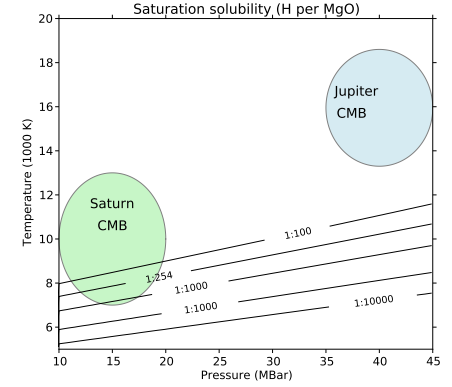
\includegraphics[scale=0.65]{../Figures/wilson_solubility.png}
\end{figure}

% cite doi:10.1088/1742-6596/717/1/012082 (Sterne et al., equations of state for ablator materials in inertial confinement fusion simulations) on the pressure ionization stuff
% cite Weir et al., Metallization of Fluid Molecular Hydrogen at 140 GPa
% cite Ebeling and Richert, PLASMA PHASE TRANSITION IN HYDROGEN 
%(cite koenig et al, doi: http://dx.doi.org/10.1088/0741-3335/47/12B/S31)
% other questions: is convection possible in the metallic H core, etc., see pg 91 of x-games

Another case in which the material properties of warm dense matter determine the behavior of an astrophysical object is that of white dwarves, whose envelopes consist of a hot, partially Fermi-degenerate plasma. Modeling the cooling of white dwarves is a topic of interest (cites), especially in the context of the importance of type 1a supernovae as `standard candles' for measuring distances to distant galaxies. Doing so, however, requires knowledge of stellar envelope opacities, equations of state (EOS), and transport properties, many of which properties are currently unknown to within factors of order unity. The absence of understanding of the simplest available system--the hydrogenic one-component plasma--underscores the difficulty of this thread of research.
% cites needed, see pg 58 of x-games

\subsection{Inertial Confinement Fusion}
The effort to reach controlled fusion through implosion of deuterium-tritium fuel capsules--an approach termed inertial confinement fusion--has progressed significantly in the last decade due to completion of laboratory facilities capable of producing HED (definition?) plasmas with densities and temperatures approaching levels needed for ignition. Fig. (which figure) shows a schematic of an ignition technique called indirect drive. In this configuration the ICF target, which consists of a hollow spherical capsule of ablator material filled with deuterium-tritium fuel, is confined in a hollow capsule of a high-Z material (the Hohlraum). A multi-TW, ns-duration duration laser passes through apertures in the Hohlraum and heats the Hohlraum to blackbody temperatures on the order of several hundred eV. The resulting thermal spectrum of soft X rays isotropically heats and ablates the fuel capsule's surface, causing its interior to implode by conservation of momentum. Typical parameters of the plasma created at maximum compression include areal densities (capsule density x radius) of 0.3 g/cm$^2$ and temperatures of the order 10 keV. (cite. see x-games pg 113)

\begin{figure}[h] \label{fig:icf}
\caption{Schematic of indirect-drive inertial confinement fusion shot. (cite)}
%(cite https://lasers.llnl.gov/science/icf/how-icf-works)}
\centering
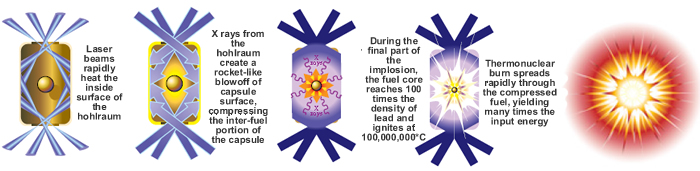
\includegraphics[scale=0.5]{../Figures/indirect-drive.jpg}
\end{figure}

Although its end state falls well within the regime of a classical plasma, the fuel capsule transitions through the WDM state during compression. The opacity and EOS of warm dense matter therefore has a strong influence on the development and propagation of shocks during ablation of the fuel capsule, which in turn affects the optimization of various experimental parameters, including fuel capsule geometry and temporal profile of the laser driver. Accurate modeling of the fuel capsule's transport properties under the WDM regime is equally important for understanding the development during compression of hydrodynamic instabilities, which are known to be a major obstacle to the efficient coupling of laser energy into fuel compression (cites).
% cite doi:10.1088/1742-6596/717/1/012082 (Sterne et al., equations of state for ablator materials in inertial confinement fusion simulations)
%TODO: cite D A Callahan, D E Hinkel, R L Berger on NIF Hohlraum temperature
% don't necessarily cite, but saumon et al. 1995 is a good reference on EOS modeling approaches.
% TODO: can say more about ICF if extra length is needed

\section{Experimental Generation of WDM}
Sentence or two here.... 
\subsection{Long-pulse lasers}
Lasers with pulse durations on the order of nanoseconds and energies of 1 kJ or more are among the most versatile tools for producing high energy density states, including warm dense matter. In the most common use cases of long pulse lasers the target is a bulk material, and coupling of laser energy into it occurs in two stages. First, the laser rapidly (TODO how rapidly) generates a coronal plasma at the material's surface. Once the electron density of this plasma exceeds the laser wavelength's critical density (TODO: equation) the laser becomes electromagnetically shielded from the material's interior and can no longer transfer energy to it. In the context of direct drive (where the material is a target to which laser energy is directly coupled), subsequent energy transfer occurs by thermal conduction of energy from the surface plasma to higher-density regions as well as by compression of the target resulting from ablation of its surface. In the case of indirect drive, the laser's energy is used to heat a surface (typically the interior of a Hohlraum) that provides a thermal bath which, in turn, couples to the target via its blackbody radiation. 

The ns duration of long-pulse lasers matches the timescale on which mechanical and hydrodynamic processes occur on typical target scales. Long-pulse lasers are thus suited to generating ramp and shock compression, notably including for the application of ICF. The largest-scale laser plasma facilities--Omega EP at the Laboratory for Laser Energetics in Rochester, NY and the National Ignition Facility--are long-pulse laser systems targeted toward the ICF program.

% TODO: pull stuff on tie-in with ICF from Brian's thesis

\subsection{Short-pulse lasers}
Short pulse lasers are a second class of systems used to generate HED conditions. They are typically defined by pulse durations on the order of a picosecond or less, down to as little as $\sim$1 fs. 

% TODO: what applications do short pulse lasers excel at?
Short-pulse laser systems arose after the development of chirped pulse amplification in the 1980s (cite) and have proliferated ever since (cites), especially with the recent advent of compact (university laboratory-scale) versions with tens of Joules of pulse energy, sufficient to generate scientifically interesting HED conditions. The largest-scale short pulse lasers have pulse powers up to 100 TW (check this number), with durations between 10 and 100 fs (check this as well).

Due to the smaller total energies of short-pulse lasers and the relatively slow cooling timescale of materials heated above ambient conditions \textit{regardless} of the pump duration, short-pulse lasers are used to generate HED conditions under direct-drive configurations alone. Energy is coupled into a target indirectly (as is the case with long-pulse systems) via `hot' MeV-scale electrons generated in the laser's interaction with plasma at the target surface. In the (typical) case where bulk heating is required, the target thickness is small compared to the hot electrons' stopping range, causing them to reflux through the target once it acquires net positive charge. This process lasts on the order of one ps (check this, cite Nilson and maybe others) and thus sets the time resolution of experiments in which the short-pulse laser is used to both heat and probe the target.

\label{foobar}
\subsection{X-Ray Free Electron Lasers}
The advent of X-Ray Free Electron lasers is a major advance in capability for WDM research. Existing incarnations of these sources, notably the Linac Coherent Light Source (LCLS), provide $10^{14}$ photons in a $\geq 10$ fs-duration monochromatic pulses with tunable energy. While the energies per pulse are smaller than those attainable with a short-pulse laser, they are largely sufficient to produce HED states with temperatures in excess of 100 eV (cite). Because XFELs can heat volumetrically, they are free of the primary deficiency of lasers with respect to the task of generating dense plasmas: namely, the latter can only heat bulk materials indirectly and over durations of 1 ps or longer, which exceeds the timescale for changes in WDM, preventing the study of short-lived transient states.

The ability to generate (and probe) WDM on truly inertial timescales, wherein atomic nuclei are effectively frozen, has been duly exploited in early pioneering studies at the LCLS. It forms the basis, for example, for a new thread of materials science research on nonthermal lattice and spin dynamics (cite Lee and others). Likely even more significantly, it is the enbling feature for macromolecular crystallography under the `diffract before destroy' paradigm. (cites) The possibilities surrounding rapid generation of WDM is a topic to which I return in (which chapter?). (cite Vinko et al. and other early LCLS papers).

% TODO: insert figure Brightness_overview.jpg and cite doi:10.1038/nphoton.2007.76
% cite Richard W. Lee, Stephen J. Moon, and Hyun-Kyung Chung 2003
% cite Lee Non-thermal dynamics of the spin and charge order in striped nickelates

\section{X-ray diagnostics of WDM}
Experimental studies of WDM suffer from a substantial complication: the opacity of WDM to photons is large at energies up to the soft X ray regime. As mentioned in section \ref{foobar}, in the context of laser heating this is merely a frustration; for the purposes of measuring the conditions of a bulk WDM system, however, the need for direct detection of radiation originating from the target's interior makes optical probes wholly ineffective. Determination of the structure and thermodynamic state variables of a dense plasma therefore requires sufficiently penetrating radiation; for this reason, the large majority of WDM diagnostics are X ray photon-in photon-out measurements. 

In the remainder of this section I provide an overview of the various available X-ray techniques.
% TODo: more text...
% TODO: plot of opacity vs T and rho, or somehting like that

\subsection{Scattering}
Elastic scattering and nonresonant inelastic X-ray scattering (NIXS) are among the most-frequently probed signals for inferring the structure, temperature and ionization state of WDM. In dense plasmas generated by long-pulse lasers, where LTE is commonly assumed, NIXS also serves as a probe of temperature.

For a given sample, the sum of scattering interactions is characterized by the double-differential scattering cross section (DDCS) $d^2\sigma/d\Omega d\omega$, which describes the probability of a photon to scatter into a solid angle increment $d\Omega$ within an energy loss interval $d\omega$. Within the independent-electron and first Born approximations the DDCS is given by

\label{ddcs}
\begin{equation}
\frac{d^2\sigma}{d\Omega d\omega} = r_0^2 (\frac{\omega_2}{\omega_1}) |\epsilon_1 \times \epsilon_2^*|^2 S(\vec{q}, \omega),
\end{equation}

where 


\label{sofq}
\begin{equation}
S(\vec{q}, \omega) \equiv \sum_F  \sum_j\langle F|  exp(i \vec{q} \cdot \vec{r}_j) |I\rangle |^2 \delta(E_F - E_I - \hbar \omega).
\end{equation}

The first term in equation \ref{ddcs} is the Thomson cross section, which describes the interaction between a probe photon and a single electron; $S(\vec{q}, \omega)$ is referred to as the dynamic structure factor, and encapsulates all system-specific properties. $I$ and $F$ are initial and final states of the sample with energies $E_I$ and $E_F$, respectively, and the second summation of \ref{sofq} is over electrons in the scatterer.

Following Chihara (cite Chihara), the typical treatment of a dense plasma separates the dynamic structure factor into several components:

\begin{equation}
S(\vec{q}, \omega) = |f_I(q) + f_e(q)|^2 S_{ii}(q, \omega) + S_{ff}(q, \omega) + S_{bf}(q, \omega),
\end{equation}

$S_{ii}$ is the atomic/ionic structure factor, $f_I$ and $f_e$ are the form factors for the ion and a surrounding cloud of screening scharge. $S_{ff}$ contains scattering from free, delocalized electrons, and $S_{bf}$ represents Raman-type bound-free transitions resulting from scattering from tightly-bound core level electrons. Note that spherical symmetry has been assumed: all terms of the structure factor depend only on the magnitude of $\vec{q}$.

The first term corresponds to elastic ($\omega = 0$) scattering, and is connected to the dense plasma's pair distribution function by a Fourier transform. Though not a component of the NIXS signal, it must often be considered in simulations and analyses of NIXS data, wherein the Bethe sum rule (cite) and other conserved quantities consist of integrals over the entire energy-loss domain of the dynamic structure factor. Elastic scattering is a highly-useful probe of structure; we consider it separately in section \ref{coh}. 

The free-free contribution to $S(q, \omega)$ can be expressed in terms of the free-electron dielectric function $\epsilon(q, \omega)$  via the fluctuation-dissipation theorem (cite Kubo et al.):

\begin{equation}
S(q, \omega) = \frac{\epsilon_0 \hbar q^2}{\pi e^2 n_e} \frac{1}{1 - e^{\hbar \omega/k_B T_e}} Im\frac{1}{\epsilon(q, \omega)},
\end{equation}

The random phase approximation (RPA) (cite Bohm and Pines) is typically used as an approximation for $\epsilon(q, \omega)$, but more recent treatments incorporate a perturbative treatment of electron-ion interactions using the Born-Mermin Approximation (cite Mermin). As shown in Fig. (which figure?), the scattering contribution of $S_{ff}$ consists of a pair of Plasmon peaks with opposite, equal-magnitude energy offsets from the elastic scattering peak. Electron density is inferred from the magnitude of the Plasmon peak shifts while temperature is obtained from the ratio of intensities of the two peaks, following the principle of detailed balance (cite Glenzer 2007 and Lee 2009).
% R Kubo.  The fluctuation-dissipation theorem.  Reports on Progress in Physics, 29(1):255, 1966.
% David Bohm and David Pines. A collective description of electron interactions: Iii.  coulomb interactions in a degenerate electron gas. Phys. Rev., 92:609–625, Nov 1953.
%N. D. Mermin. Lindhard dielectric function in the relaxation-time approximation.  Phys. Rev. B, 1:2362–2363, Mar 1970.
% figure comes from Lee 2009

Although the connection of temperature and density to the free-free component of the dielectric function is well-founded, there are two obstacles to effective interpretation of collective scattering data from WDM systems; one is theoretical and the other experimental. First, the validity of established treatments of the dielectric function has been called into question, with recent plasmon spectrum calculations based on MD-DFT simulations showing a significant change in the plasmon profile compared to that predicted by the BMA. (cite Mattern thesis and Plagemann). Second, the plasmon peak suffers from poor signal to background and has a small separation from the elastic scattering peak under typical WDM electron densities, making it difficult to resolve. As a result only a handful of experiments to date have pursured this technique. 

We finally turn our attention to the last term of \ref{sofq}, $S_{bf}$, whose contribution to the inelastic DDCS is often referred to as x-ray Thomson scattering (XRTS). Obtaining state variable information from a system's bound-free scattering contribution is dependent on the underlying model of electronic structure used; as a result, various treatments exist, including the Impulse Approximation (IA) of Eisenberger and Platzman, wherein the bound-free contribution to XRTS is equivalent to Doppler-broadened Compton scattering (cite Eisenberger and Platzman); the plane wave form factor approximation (PWFFA) of Schumacher (cite Schumacher), which attempts to extend the IA by incorporating electron binding energies; and calculation of matrix elements using a real space Green's function (RSGF) formalism applied to atomic clusters, as implemented in the atomic spectroscpy code FEFF (cite Mattern).

% TODO: need to track down the paper...
%\begin{figure}[h] \label{fig:lee}
%\caption{}
%\centering
%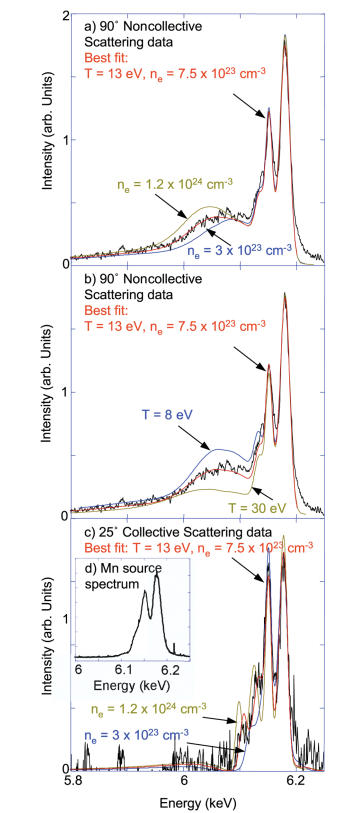
\includegraphics[scale=0.5]{../Figures/lee_xrts.png}
%\end{figure}

In current practice, measurement of the  bound-free component of XRTS from WDM is performed in the large-$q$ regime, where the Compton feature is broad and can be measured using high-efficiency (but low-resolution) HOPG-based spectrometers (need cites for this). As such, single-particle bound-free scattering is more readily measured than collective excitation features. Since an early demonstration of the technique by Glenzer et al. (cite Glenzer 2003) it has been frequently implemented at both laser plasma and XFEL facilities (cite figures showing how these experiments are set up). Despite some fruitful outcomes (how so? need examples, cites), the large statistical uncertainties in XRTS spectra--particularly at laser plasma facilities, where single-shot measurements are photon-starved--make the inference of state variables difficult, and dependent on one's choice of electronic structure model (check that this is right. do predicitons heavily depend on the choice of model, or is it just that uncertainties are high, regardless of the choice?). Mattern et al. have demonstrated this concretely by comparing theoretical fits to XRTS data of shock-compressed Be, and argue that the lack of rigorous validation of electronic structure models for WDM models strongly undermines their validity for first-principles measurement of state variables. With this context as motivation, we revisit the topic of WDM thermometry in chapter (reference chapter).
% S. H. Glenzer, G. Gregori, F. J. Rogers, D. H. Froula, S. W. Pollaine, R. S. Wallace, and O. L. Landen. X-ray scattering from solid density plasmas. Physics of Plasmas, 10(6):2433–2441, 2003.
% TODO fix the terminology here. Does XRTS refer to just bound-free contribution (don't think so)

\label{coh}
\subsection{Coherent Scattering}
Coherent scattering is the zero-energy loss component of the double differential cross section.  The inference of structural information from coherent scattering varies by material; two primary cases present themselves.

%, consisting of the contribution of terms in equation \ref{sofq} with  $\langle I| = \langle F|$. From equation \ref{sofq} ts differential cross section $d\sigma_{coh}/d\Omega$ has the simple proportionality
%
%\begin{equation}
%\frac{d\sigma_{coh}}{d\Omega} \propto \Sigma_j exp(i \vec{q} \cdot \vec{r}_j) 
%\end{equation}
%finish this..............


First, for amorphous materials, such as hot dense plasmas generated by ramp- or shock-compression and lacking long-range order, the scattering amplitude is isotropic and is characterized by the one-dimensional static structure factor, which is connected by a Fourier transform to the material's pair correlation function. Inference of the full pair correlation function is in practice frustrated by the difficulty of inverting a limited momentum transfer range-sampling of the strucure factor, but even in the most information-limited scenarios a density can nevertheless be recovered from the strucure factor's first correlation peak. Although coherent scattering measurements from dense plasmas have been demonstrated in the context of long-pulse laser compression experiments, implementation difficulties unique to that environment prevent its adoption as a routine techique. We address these difficulties, and proposed solutions, in chapter (chapter reference). (cite Ma et al).

Second, in materials with long-range crystalline order, as typically found in XFEL-based experiments (whose timescales are shorter than the thermalization rate of electronic and ionic degrees of freedom), the coherent scattering amplitude is given by

\begin{equation}
F(\vec{q}) = \Sigma_n e^{i \vec{q} \cdot \vec{R_n}} \Sigma_j f_j(\vec{q}) e^{i \vec{q} \cdot \vec{r_j}},
\end{equation}

where the first summation is over all lattice vectors $\vec{R_n}$ and the second, reffered to as the \emph{unit cell structure factor}, is over postions $\vec{r_j}$ of atoms within the unit cell. By the convolution theorem, the crystal's scattering amplitude in reciprocal space is equal to the product of the lattice and unit cell structure factor. The coherent scattering signal is therefore a discrete sampling of the unit cell structure factor at individual Bragg peaks with momentum transfers corresponding to vectors of the reciprocal lattice.

\begin{figure}[h] \label{fig:ma}
\caption{Experimental elastic scattering intensity of shock-compressed Al at OMEGA-60, compared to several hypernetted chain (HNC), Debye-Hueckel (DH), and screened one-component plasma (SOCP) models. (cite Ma et al.)}
%(cite https://lasers.llnl.gov/science/icf/how-icf-works)}
\centering
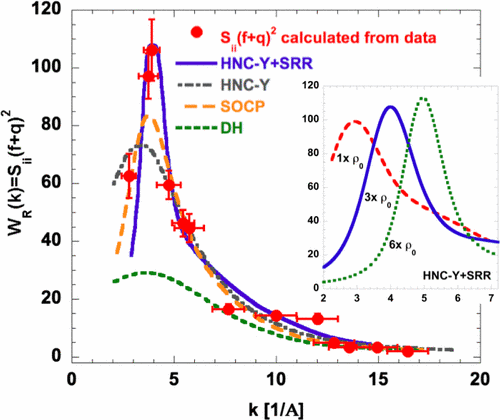
\includegraphics[scale=0.5]{../Figures/ma_Al.png}
\end{figure}

In the context of XRD from a material undergoing thermalization under fs XFEL heating, the crystal scattering amplitude's decomposition into lattice and unit cell components has a direct correspondence to interpretation of structural change. The onset of long-range lattice disorder is readily identifiable as a quenching in Bragg peaks roughly proportional to $e^{-q^2}$. Evolution of the unit cell structure factor, on the other hand, is dependent on the details of atomic level populations and the material's finite-temperature electronic structure, and can be used as a test of competing theoretical models of both. 

(need cites and discussion of the existing literature on XRD of XFEL-heated WDM)




\subsection{X-ray absorption}
X-ray absorption spectroscopy (XAS) may be used to measure the structure and unoccupied electronic density of states of WDM systems. The information available by X-ray absorption near-edge spectroscopy (XANES) and X-ray absorption fine structure (XAFS) is the same as in other scientific contexts, but the experimental implementation differs in a few respects. In all instances, the short duration of WDM states requires instantaneous collection of absorption spectra using a source with broad-band spectrum. At laser plasma facilities this is arranged using a spherical capsule of CH polymer imploded using a long-pulse laser (cite yaakobi 2003) that emits a thermal spectrum with a \textbackslash 1 MeV temperature (check this). This so-called broadband backlighter has been used to collect XAFS for the study of compression-induced phase transitions, such as that from bcc to hcp Fe driven by ns shock-comression (cite Yaakobi 2005).

\begin{figure}[h] \label{fig:xafs}
\caption{FEFF calculation of XAFS for hcp and bcc phases of Fe (a), compared to experimental data taken on ambient and shock-compressed Fe at the OMEGA laser (b). (cite Yaakobi)}
%(cite https://lasers.llnl.gov/science/icf/how-icf-works)}
\centering
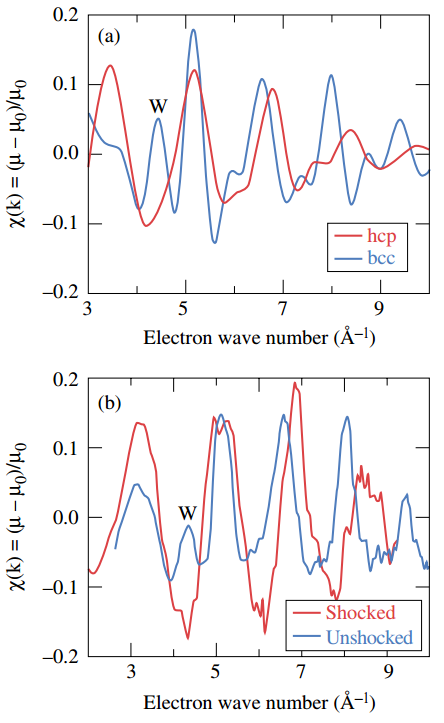
\includegraphics[scale=0.6]{../Figures/yaakobi_shock_xafs.png}
\end{figure}

XANES measurements on dense plasma have also been performed at laser plasma facilities. This requires narrower-band illumination compared with XAFS, which has been achieved using short pulse laser-driven multicomponent X-ray fluorescence backlighters. Levy et al., for example, have used this technique to demonstrate XANES-based thermometry based on measurement of the K-edge slope in Al isochorically heated to 3 eV. (cite Levy et al).

Laser wakefield accelerator X-ray sources generate fs-duration broadband X-ray emission, affording time resolution that surpasses what is possible with laser-driven backlighters. This makes wakefield accelerators especially well-suited to X-ray absorption spectroscopy of WDM generated at XFEL facilities (cite Albert). The combination of wakefield accelerators with XFELs promises the unprecented possibility of XFEL pump-probe experiments with simultaneous fs-duration interrogation of the target using broad- and narrow-band hard X-rays. This combination also enables XAS measurements of low-Z materials, which is much more challenging at laser plasma facilities as a result of the mismatch between the short penetration lengths of x-rays near the K-edges of low-Z species and the relatively large target thicknesses (tens of microns) needed for effective laser ablation. 
% TODO  this paragraph sucks. 
% One appealing possibility is that of simultaneous XAS and XRD.
% TODO: use the figure from Albert et al.


\subsection{X-ray Emission and X-ray Fluorescence}
X-ray fluorescence spectroscopy (XRF) is an extensively used probe in experiments studying the interaction of high-intensity lasers with solid targets. In short-pulse laser experiments involving mid-Z elements heated to temperatures comparable to or larger than M-shell binding energies the ratio of $K_\beta$ to $K_\alpha$ emission is used as a measurement of temperature. Modeling the coupling efficiency between high-power laser and electrons in a solid-density target is of considerable significance to the effort to understand optical radiation-matter interactions at high laser intensities ($> 10^{19}$ W/cm$^2$); in this context, inference of target heating using $K_\beta/K_\alpha$ branching ratios provides a useful consistency check in the application of models to experimental data. (cite Myatt et all 2007, Nilson).

\begin{figure}[h] \label{fig:nilson}
\caption{Experimental $K_\alpha/K_\beta$ ratios of emission from Cu foil heated by short-pulse lasers, with inferred electron temperature on the right vertical axis. Model calculations are heating for hot electron coupling efficiencies $\eta_e$ equal to 10\% and 30\% (cite Nilson)}
%(cite https://lasers.llnl.gov/science/icf/how-icf-works)}
\centering
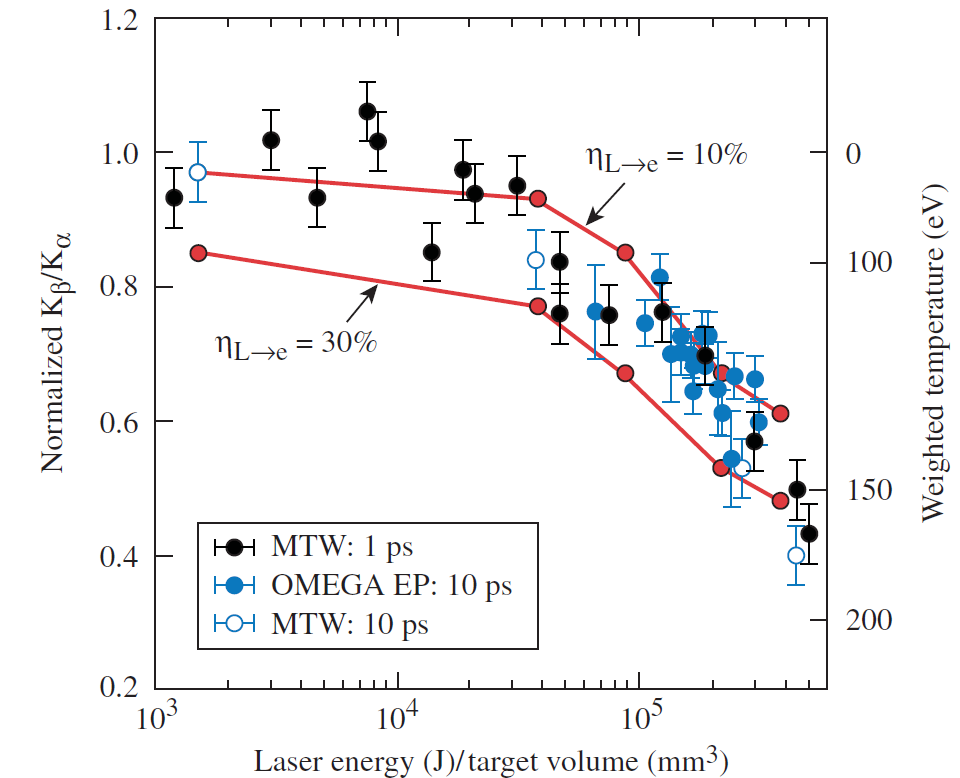
\includegraphics[scale=0.5]{../Figures/nilson_branching.png}
\end{figure}

X-ray emission spectroscopy (XES), the finer-grained cousin of XRF, provides more detailed information on the occupied density of states in a material and can be sensitive to valence-level excitations in the `tepid' transitional regime between ambient and warm dense matter states (reference XES figure from the LD67, maybe get some cites). It has seen use primarily at XFEL facilities, where higher shot rates and probe intensities make the collection of datasets with satisfactory statistical quality easier. (cite photosystem 2 XES papers). The advent of XFELs as the first high-intensity, monochromatic, and tunable WDM probes has also enabled resonant inelastic X-ray scattering (RIXS) measurements, which has made possible the direct measurement of ionization potential depression on a fs timescale, as demonstrated by Vinko et al. (cite Vinko, Ciricosta.).

% K-U Plagemann, P Sperling, R Thiele, M P Desjarlais, C Fortmann, T D ̈oppner, H J Lee, S H Glenzer, and R Redmer. Dynamic structure factor in warm dense beryllium.  New Journal of Physics, 14(5):055020, 2012.


%In the high-momentum transfer Impulse Approximation of Eisenberger and Platzman, for example, XRTS becomes equivalent to Doppler-broadened Compton scattering, wherein the DDCS is proportional to an integral over the system's momentum-space density $\rho(p)$:
%
%\begin{equation}
%	\frac{d^2\sigma}{d\Omega d\omega} \propto \int d^3p \rho(p) \delta(p_q - (\omega m / q - \hbar q / 2)).
%\end{equation}
% TODO figure out what to do with section. How much detail is needed.


	% TODO: latex vectors?
	% TODO: cites. use either brian's thesis or same source as in the edxrd paper

	%The fundamental observable of XRTS is the dynamic structure factor $S(q, \omega)$ 


\section{Dissertation Outline}
The overaching theme in this thesis is the relationship, and frequent feedback, between scientific discovery and the development of new experimental techinique. To begin, in chapter 2 I introduce a scheme for single-shot measurement of the static structure factors of disordered dense plasmas produced at large-scale laser facilities such as Omega and NIF. In Chapter 3 I present an experimental observation of nonlocal heat transport by keV-scale electrons in a nanophase material and consider the question of how this effect can be used to improve WDM experiments conducted at XFELs via optimized nanostructured target design. In chapter 4 I discuss experimental results of a recent experiment at the LCLS in which we established bounds on the timescales for thermalization of the lattice in XFEL-heated metal oxides and measured the consequences of XFEL heating on electronic charge density, with subsequent comparisons to different model predictions.  In chapter 5 I describe an instrument-development effort toward a disposable CMOS-based X-ray camera for use in experimental environments hostile to electronics, particularly laser plasma facilities. Finally, in chapter 6 I introduce UW-XAP, a software tool for streamlined realtime data collection and analysis at the LCLS. 



 
% Chapter 1

\chapter{Chapter Title Here} % Main chapter title

\label{Chapter1} % For referencing the chapter elsewhere, use \ref{Chapter1} 

%----------------------------------------------------------------------------------------

% Define some commands to keep the formatting separated from the content 
\newcommand{\keyword}[1]{\textbf{#1}}
\newcommand{\tabhead}[1]{\textbf{#1}}
\newcommand{\code}[1]{\texttt{#1}}
\newcommand{\file}[1]{\texttt{\bfseries#1}}
\newcommand{\option}[1]{\texttt{\itshape#1}}

%----------------------------------------------------------------------------------------

%Outline for this section.
%Context: splice this section into the HEF paper as part of an extended
%methods section. Before talking about PENELOPE I need to state what it
%is that we need to model, and with what accuracy.
%1. Summarize what PENELOPE is.
%2. PENELOPE's treatment of elastic scattering and how it satisfies our requirements. How much detail can I omit here? For example, treatment of the 
%3. PENELOPE's treatment of inelastic scattering, including the Liljequist GOS model, and how it satisfies our requirements. 
%4. PENELOPE's treatment of the material-dependent energy-loss function.
%Discuss the program MATERIAL and justify penelope's use of Bragg's rule.
%May need to discuss the estar database?
Elastic scattering of electrons refers to interactions do not alter target atoms' states. Above energies of a few hundred eV it may be described as an interaction between an electron and a target atom's electrostatic field (static field approximation. Cite Mott and Masse 1965). The atom's electrostatic potential is expressed in terms of the nuclear and electronic charge densities $\rho _n (r)$ and $\rho _e (r)$, respectively:

\begin{amsmath}
\phi (r) = e~4~\pi [\frac{1}{r}\int_0^{r}\rho(r')r'^{2} + \int_r^{\infty}\rho_n(r')r'dr'] - e~4~\pi \frac{1}{r} \int_0^r\rho_e(r')r'^2 dr' + \int_r^\infty \rho_e(r') r' dr'].
\end{amsmath}
At the energy scales of the simulations described in chapter (which chapter?) the nucleus may be considered a point charge, but PENELOPE accounts for the effect of the finite nuclear size on the high-energy (> MeV) elastic DCS with the following approximation using the Fermi distribution:

\begin{equation}
\rho_n(r) = \frac{\rho_0}{exp[(r - R_n)(4ln3/t)] + 1},
\end{equation},

(cite Hahn et al. 1956 and understand the orgin of this expression)  $R_n$ is the mean radius and $t$ is the 'skin` thickness of $\rho_n$ defined in Hahn et al. 1956. 

The total interaction energy for electrons is

\begin{equation}
V(r) = -e\phi(r) + V_{ex}(r),
\end{equation}

where $V_{ex}(r)$ is a local approximation of the exchange interaction. The angular distribution of elastic scattering off this central field is axially symmetric, and the DCS $d\sigma_{el}/d\Omega$ may therefore be expanded into a sum of Legendre polynomials. [Citing Salvat 2005 or Walker, describe how the phase shifts are obtained from the Dirac radial wave functions. What's the role of the exchange term in all this?]

\section{First view: Yukawa potential}
The Yukawa potential,

\begin{equation}
V(r) = \alpha^2 \frac{e^{-\mu r}}{r}
\end{equation}

is a crude description of an atomic potential that is nevertheless sufficient to derive the approximate differential cross section of elastic scattering and to describe its influence on the spatial distribution of scattered electrons at our energy scale of interest. 

The first Born approximation gives the amplitude for a particle's scattering off of a spherically symmetric potential as

\begin{equation}
f(\theta) \simeq -\frac{m}{2\pi \hbar^2} \int e^{i q r_0 cos \theta_0 sin \theta_0 d\theta_0
\end{equation}

Substituting (how do I reference equations) into (), yields 
%from http://itp.uni-frankfurt.de/~valenti/SS14/QMII_2014_chap1.pdf
%TODO: make the notation here consistent.
\begin{equation}
\begin{split}
f(\theta)  \simeq -\frac{2m\alpha^2}{\hbar^2q} \int_0^\infty e^{-r \mu} sin(q r) dr = -\frac{2m\alpha^2}{\hbar^2 (\mu^2 + q^2)} \\
& \frac{4 Z^2}{a_0^2 k_0^4} \frac{1}{(\theta^2 + \theta_0^2)^2},
\end{split}
\end{equation}
where $\theta_0 = (k_0 r_0)^{-1}$ is the characteristic angle for elastic scattering.

Integrating over scattering angles gives
\begin{equation}
\sigma_e = \int_0^\pi \frac{d\sigma}{d\Omega} 2 \pi sin \theta d \theta = \frac{4 \pi}{k_0^2} Z^{4/3}
\end{equation}

For 10 keV electrons $\theta_0 = $ how much??? and $\sigma_e = $ how much???. Taking the atomic number of density of Fe, the mean free path between inelastic collisions is (insert the right expression) = (insert the right number). The corresponding expectation value of angular deflection per distance traveled is (insert the right number). In comparison, the inelastic mean free path of 10 keV photons in Fe (potential see-saw here is (insert number). where should i introduce inelastic scattering?) This suggests that path deflections caused by elastic scattering will have a significant influence on the spatial distribution of energy deposited 10 keV-scale electrons in Fe and other mid-Z materials. 


Fig. (fig reference) shows the angular dependence of scattering for Fe. 

\section{Inelastic scattering}
Inelastic collisions are the dominant mechanism for energy loss of electrons up to (how many keV?) (reference figure with plot of cross secions as a function of energy)
%The double differential cross section for collisions with momentum transfer $q$ and energy loss $\omega$ is given by Fano (cite Fano 1963, see page 114 of PENELOPE manual) as

In an atomic system, the differential cross section for a transition from initial state wavefunction $\psi_0$ to final state wavefunction $\psi_n$ is

\begin{equation} \label{bornDCS}
\frac{d\sigma_n}{d\Omega} = (\frac{m_0}{2\pi \hbar^2}^2 \frac{k_1}{k_0} \mid \int V(r) \psi_0 \psi_n* exp(i q r) d\tau \mid ^2
\end{equation}
%TODO: fix the notation here. How does one do bolded text? dot products?
where $\textbf{k}_0$ and $\textbf{k}_1$ are the wave vectors of the incident electron before and after scattering and $q = \hbar (\textbf{k}_1 - \textbf{k}_1)$ is the corresponding momentum transfer. 

For electron energies below 300 keV (elaborate on how this breaks down) the potential between electron and atom may be expressed as the sum of Coulomb potentials of the nucleus and atomic electrons:

\begin{equation} \label{cpotential}
V(r) = \frac{Ze^2}{4\pi \epsilon_0 r} - \frac{1}{4 \pi \epsilon_0} \sum_{j = 1}^Z \frac{e^2}{\mid \textbf{r} - \textbf{r_j} \mid}
\end{equation}
%TODO
%(explain here why the nuclear potential term drops out in the integral)
%TODO
%(define whichever quantities haven't been introduced yet)
Substituting the second term of equation \ref{cpotential} into \ref{bornDCS} gives the following expression for the differential cross section of inelastic scattering: 

\begin{equation} \label{inelasticDCS}
\frac{d\sigma_n}{d\Omega} = (\frac{4 \gamma^2}{a_0^2 q^4}) \frac{k1}{k0} \mid \epsilon(q)\mid^2,
\end{equation}

where

\begin{equation}
\epsilon_n = \int \psi_n* \sum_j exp(i q r_j) \psi_0 dd\tau.
\end{equation}

We note that PENELOPE incorporates Fano's (1963) relativistic treatment of inelastic scattering of electrons in condensed media in place of the current treatment. 
equation \ref{inlasticDCS}. 
Because this simplified treatment is equivalent in our regime of interest (scattering of $< 100eV$ electrons), (citation needed?) we confine the current discussion to 

The generalized oscillator strength is an important related quantity:

\begin{equation}
f_n(q) = \frac{E_n}{R} \frac{\mid \epsilon_n(q)\mid ^2}{(q a_0)^2},
\end{equation}


where $R = (m_0 e^4 / 2)(4 \pi \epsilon_0 \hbar)^{-2}$, the Rydberg energy, and $E_n$ is the energy change of the transition. 

Because the energy-loss spectrum is in general continuous it is customary to describe inelastic scattering by a double-differential cross section:

\begin{equation} \label{inelastic_DDCS}
\frac{d^2\sigma}{d\Omega dE} = {4 \gamma^2 R}{Eq^2} \frac{k_1}{k_0} \frac{df}{dE}(q, E)
\end{equation}

The GOS per unit energy loss is the central quantity which, within the first Born approximation, fully determines the scattering cross section.  and 

%TODO: introduce the GOS in the first expression for the DDCS.


NOTES:
See appendix a in Egerton for justification of the simplified interaction potential for an incident electron and an atom below 300 keV. 


%\section{Welcome and Thank You}
%Welcome to this \LaTeX{} Thesis Template, a beautiful and easy to use template for writing a thesis using the \LaTeX{} typesetting system.
%
%If you are writing a thesis (or will be in the future) and its subject is technical or mathematical (though it doesn't have to be), then creating it in \LaTeX{} is highly recommended as a way to make sure you can just get down to the essential writing without having to worry over formatting or wasting time arguing with your word processor.
%
%\LaTeX{} is easily able to professionally typeset documents that run to hundreds or thousands of pages long. With simple mark-up commands, it automatically sets out the table of contents, margins, page headers and footers and keeps the formatting consistent and beautiful. One of its main strengths is the way it can easily typeset mathematics, even \emph{heavy} mathematics. Even if those equations are the most horribly twisted and most difficult mathematical problems that can only be solved on a super-computer, you can at least count on \LaTeX{} to make them look stunning.
%
%%----------------------------------------------------------------------------------------
%
%\section{Learning \LaTeX{}}
%
%\LaTeX{} is not a \textsc{wysiwyg} (What You See is What You Get) program, unlike word processors such as Microsoft Word or Apple's Pages. Instead, a document written for \LaTeX{} is actually a simple, plain text file that contains \emph{no formatting}. You tell \LaTeX{} how you want the formatting in the finished document by writing in simple commands amongst the text, for example, if I want to use \emph{italic text for emphasis}, I write the \verb|\emph{text}| command and put the text I want in italics in between the curly braces. This means that \LaTeX{} is a \enquote{mark-up} language, very much like HTML.
%
%\subsection{A (not so short) Introduction to \LaTeX{}}
%
%If you are new to \LaTeX{}, there is a very good eBook -- freely available online as a PDF file -- called, \enquote{The Not So Short Introduction to \LaTeX{}}. The book's title is typically shortened to just \emph{lshort}. You can download the latest version (as it is occasionally updated) from here:
%\url{http://www.ctan.org/tex-archive/info/lshort/english/lshort.pdf}
%
%It is also available in several other languages. Find yours from the list on this page: \url{http://www.ctan.org/tex-archive/info/lshort/}
%
%It is recommended to take a little time out to learn how to use \LaTeX{} by creating several, small `test' documents, or having a close look at several templates on:\\ 
%\url{http://www.LaTeXTemplates.com}\\ 
%Making the effort now means you're not stuck learning the system when what you \emph{really} need to be doing is writing your thesis.
%
%\subsection{A Short Math Guide for \LaTeX{}}
%
%If you are writing a technical or mathematical thesis, then you may want to read the document by the AMS (American Mathematical Society) called, \enquote{A Short Math Guide for \LaTeX{}}. It can be found online here:
%\url{http://www.ams.org/tex/amslatex.html}
%under the \enquote{Additional Documentation} section towards the bottom of the page.
%
%\subsection{Common \LaTeX{} Math Symbols}
%There are a multitude of mathematical symbols available for \LaTeX{} and it would take a great effort to learn the commands for them all. The most common ones you are likely to use are shown on this page:
%\url{http://www.sunilpatel.co.uk/latex-type/latex-math-symbols/}
%
%You can use this page as a reference or crib sheet, the symbols are rendered as large, high quality images so you can quickly find the \LaTeX{} command for the symbol you need.
%
%\subsection{\LaTeX{} on a Mac}
% 
%The \LaTeX{} distribution is available for many systems including Windows, Linux and Mac OS X. The package for OS X is called MacTeX and it contains all the applications you need -- bundled together and pre-customized -- for a fully working \LaTeX{} environment and work flow.
% 
%MacTeX includes a custom dedicated \LaTeX{} editor called TeXShop for writing your `\file{.tex}' files and BibDesk: a program to manage your references and create your bibliography section just as easily as managing songs and creating playlists in iTunes.
%
%%----------------------------------------------------------------------------------------
%
%\section{Getting Started with this Template}
%
%If you are familiar with \LaTeX{}, then you should explore the directory structure of the template and then proceed to place your own information into the \emph{THESIS INFORMATION} block of the \file{main.tex} file. You can then modify the rest of this file to your unique specifications based on your degree/university. Section \ref{FillingFile} on page \pageref{FillingFile} will help you do this. Make sure you also read section \ref{ThesisConventions} about thesis conventions to get the most out of this template.
%
%If you are new to \LaTeX{} it is recommended that you carry on reading through the rest of the information in this document.
%
%Before you begin using this template you should ensure that its style complies with the thesis style guidelines imposed by your institution. In most cases this template style and layout will be suitable. If it is not, it may only require a small change to bring the template in line with your institution's recommendations. These modifications will need to be done on the \file{MastersDoctoralThesis.cls} file.
%
%\subsection{About this Template}
%
%This \LaTeX{} Thesis Template is originally based and created around a \LaTeX{} style file created by Steve R.\ Gunn from the University of Southampton (UK), department of Electronics and Computer Science. You can find his original thesis style file at his site, here:
%\url{http://www.ecs.soton.ac.uk/~srg/softwaretools/document/templates/}
%
%Steve's \file{ecsthesis.cls} was then taken by Sunil Patel who modified it by creating a skeleton framework and folder structure to place the thesis files in. The resulting template can be found on Sunil's site here:
%\url{http://www.sunilpatel.co.uk/thesis-template}
%
%Sunil's template was made available through \url{http://www.LaTeXTemplates.com} where it was modified many times based on user requests and questions. Version 2.0 and onwards of this template represents a major modification to Sunil's template and is, in fact, hardly recognisable. The work to make version 2.0 possible was carried out by \href{mailto:vel@latextemplates.com}{Vel} and Johannes Böttcher.
%
%%----------------------------------------------------------------------------------------
%
%\section{What this Template Includes}
%
%\subsection{Folders}
%
%This template comes as a single zip file that expands out to several files and folders. The folder names are mostly self-explanatory:
%
%\keyword{Appendices} -- this is the folder where you put the appendices. Each appendix should go into its own separate \file{.tex} file. An example and template are included in the directory.
%
%\keyword{Chapters} -- this is the folder where you put the thesis chapters. A thesis usually has about six chapters, though there is no hard rule on this. Each chapter should go in its own separate \file{.tex} file and they can be split as:
%\begin{itemize}
%\item Chapter 1: Introduction to the thesis topic
%\item Chapter 2: Background information and theory
%\item Chapter 3: (Laboratory) experimental setup
%\item Chapter 4: Details of experiment 1
%\item Chapter 5: Details of experiment 2
%\item Chapter 6: Discussion of the experimental results
%\item Chapter 7: Conclusion and future directions
%\end{itemize}
%This chapter layout is specialised for the experimental sciences.
%
%\keyword{Figures} -- this folder contains all figures for the thesis. These are the final images that will go into the thesis document.
%
%\subsection{Files}
%
%Included are also several files, most of them are plain text and you can see their contents in a text editor. After initial compilation, you will see that more auxiliary files are created by \LaTeX{} or BibTeX and which you don't need to delete or worry about:
%
%\keyword{example.bib} -- this is an important file that contains all the bibliographic information and references that you will be citing in the thesis for use with BibTeX. You can write it manually, but there are reference manager programs available that will create and manage it for you. Bibliographies in \LaTeX{} are a large subject and you may need to read about BibTeX before starting with this. Many modern reference managers will allow you to export your references in BibTeX format which greatly eases the amount of work you have to do.
%
%\keyword{MastersDoctoralThesis.cls} -- this is an important file. It is the class file that tells \LaTeX{} how to format the thesis. 
%
%\keyword{main.pdf} -- this is your beautifully typeset thesis (in the PDF file format) created by \LaTeX{}. It is supplied in the PDF with the template and after you compile the template you should get an identical version.
%
%\keyword{main.tex} -- this is an important file. This is the file that you tell \LaTeX{} to compile to produce your thesis as a PDF file. It contains the framework and constructs that tell \LaTeX{} how to layout the thesis. It is heavily commented so you can read exactly what each line of code does and why it is there. After you put your own information into the \emph{THESIS INFORMATION} block -- you have now started your thesis!
%
%Files that are \emph{not} included, but are created by \LaTeX{} as auxiliary files include:
%
%\keyword{main.aux} -- this is an auxiliary file generated by \LaTeX{}, if it is deleted \LaTeX{} simply regenerates it when you run the main \file{.tex} file.
%
%\keyword{main.bbl} -- this is an auxiliary file generated by BibTeX, if it is deleted, BibTeX simply regenerates it when you run the \file{main.aux} file. Whereas the \file{.bib} file contains all the references you have, this \file{.bbl} file contains the references you have actually cited in the thesis and is used to build the bibliography section of the thesis.
%
%\keyword{main.blg} -- this is an auxiliary file generated by BibTeX, if it is deleted BibTeX simply regenerates it when you run the main \file{.aux} file.
%
%\keyword{main.lof} -- this is an auxiliary file generated by \LaTeX{}, if it is deleted \LaTeX{} simply regenerates it when you run the main \file{.tex} file. It tells \LaTeX{} how to build the \emph{List of Figures} section.
%
%\keyword{main.log} -- this is an auxiliary file generated by \LaTeX{}, if it is deleted \LaTeX{} simply regenerates it when you run the main \file{.tex} file. It contains messages from \LaTeX{}, if you receive errors and warnings from \LaTeX{}, they will be in this \file{.log} file.
%
%\keyword{main.lot} -- this is an auxiliary file generated by \LaTeX{}, if it is deleted \LaTeX{} simply regenerates it when you run the main \file{.tex} file. It tells \LaTeX{} how to build the \emph{List of Tables} section.
%
%\keyword{main.out} -- this is an auxiliary file generated by \LaTeX{}, if it is deleted \LaTeX{} simply regenerates it when you run the main \file{.tex} file.
%
%So from this long list, only the files with the \file{.bib}, \file{.cls} and \file{.tex} extensions are the most important ones. The other auxiliary files can be ignored or deleted as \LaTeX{} and BibTeX will regenerate them.
%
%%----------------------------------------------------------------------------------------
%
%\section{Filling in Your Information in the \file{main.tex} File}\label{FillingFile}
%
%You will need to personalise the thesis template and make it your own by filling in your own information. This is done by editing the \file{main.tex} file in a text editor or your favourite LaTeX environment.
%
%Open the file and scroll down to the second large block titled \emph{THESIS INFORMATION} where you can see the entries for \emph{University Name}, \emph{Department Name}, etc \ldots
%
%Fill out the information about yourself, your group and institution. You can also insert web links, if you do, make sure you use the full URL, including the \code{http://} for this. If you don't want these to be linked, simply remove the \verb|\href{url}{name}| and only leave the name.
%
%When you have done this, save the file and recompile \code{main.tex}. All the information you filled in should now be in the PDF, complete with web links. You can now begin your thesis proper!
%
%%----------------------------------------------------------------------------------------
%
%\section{The \code{main.tex} File Explained}
%
%The \file{main.tex} file contains the structure of the thesis. There are plenty of written comments that explain what pages, sections and formatting the \LaTeX{} code is creating. Each major document element is divided into commented blocks with titles in all capitals to make it obvious what the following bit of code is doing. Initially there seems to be a lot of \LaTeX{} code, but this is all formatting, and it has all been taken care of so you don't have to do it.
%
%Begin by checking that your information on the title page is correct. For the thesis declaration, your institution may insist on something different than the text given. If this is the case, just replace what you see with what is required in the \emph{DECLARATION PAGE} block.
%
%Then comes a page which contains a funny quote. You can put your own, or quote your favourite scientist, author, person, and so on. Make sure to put the name of the person who you took the quote from.
%
%Following this is the abstract page which summarises your work in a condensed way and can almost be used as a standalone document to describe what you have done. The text you write will cause the heading to move up so don't worry about running out of space.
%
%Next come the acknowledgements. On this page, write about all the people who you wish to thank (not forgetting parents, partners and your advisor/supervisor).
%
%The contents pages, list of figures and tables are all taken care of for you and do not need to be manually created or edited. The next set of pages are more likely to be optional and can be deleted since they are for a more technical thesis: insert a list of abbreviations you have used in the thesis, then a list of the physical constants and numbers you refer to and finally, a list of mathematical symbols used in any formulae. Making the effort to fill these tables means the reader has a one-stop place to refer to instead of searching the internet and references to try and find out what you meant by certain abbreviations or symbols.
%
%The list of symbols is split into the Roman and Greek alphabets. Whereas the abbreviations and symbols ought to be listed in alphabetical order (and this is \emph{not} done automatically for you) the list of physical constants should be grouped into similar themes.
%
%The next page contains a one line dedication. Who will you dedicate your thesis to?
%
%Finally, there is the block where the chapters are included. Uncomment the lines (delete the \code{\%} character) as you write the chapters. Each chapter should be written in its own file and put into the \emph{Chapters} folder and named \file{Chapter1}, \file{Chapter2}, etc\ldots Similarly for the appendices, uncomment the lines as you need them. Each appendix should go into its own file and placed in the \emph{Appendices} folder.
%
%After the preamble, chapters and appendices finally comes the bibliography. The bibliography style (called \option{authoryear}) is used for the bibliography and is a fully featured style that will even include links to where the referenced paper can be found online. Do not underestimate how grateful your reader will be to find that a reference to a paper is just a click away. Of course, this relies on you putting the URL information into the BibTeX file in the first place.
%
%%----------------------------------------------------------------------------------------
%
%\section{Thesis Features and Conventions}\label{ThesisConventions}
%
%To get the best out of this template, there are a few conventions that you may want to follow.
%
%One of the most important (and most difficult) things to keep track of in such a long document as a thesis is consistency. Using certain conventions and ways of doing things (such as using a Todo list) makes the job easier. Of course, all of these are optional and you can adopt your own method.
%
%\subsection{Printing Format}
%
%This thesis template is designed for double sided printing (i.e. content on the front and back of pages) as most theses are printed and bound this way. Switching to one sided printing is as simple as uncommenting the \option{oneside} option of the \code{documentclass} command at the top of the \file{main.tex} file. You may then wish to adjust the margins to suit specifications from your institution.
%
%The headers for the pages contain the page number on the outer side (so it is easy to flick through to the page you want) and the chapter name on the inner side.
%
%The text is set to 11 point by default with single line spacing, again, you can tune the text size and spacing should you want or need to using the options at the very start of \file{main.tex}. The spacing can be changed similarly by replacing the \option{singlespacing} with \option{onehalfspacing} or \option{doublespacing}.
%
%\subsection{Using US Letter Paper}
%
%The paper size used in the template is A4, which is the standard size in Europe. If you are using this thesis template elsewhere and particularly in the United States, then you may have to change the A4 paper size to the US Letter size. This can be done in the margins settings section in \file{main.tex}.
%
%Due to the differences in the paper size, the resulting margins may be different to what you like or require (as it is common for institutions to dictate certain margin sizes). If this is the case, then the margin sizes can be tweaked by modifying the values in the same block as where you set the paper size. Now your document should be set up for US Letter paper size with suitable margins.
%
%\subsection{References}
%
%The \code{biblatex} package is used to format the bibliography and inserts references such as this one \parencite{Reference1}. The options used in the \file{main.tex} file mean that the in-text citations of references are formatted with the author(s) listed with the date of the publication. Multiple references are separated by semicolons (e.g. \parencite{Reference2, Reference1}) and references with more than three authors only show the first author with \emph{et al.} indicating there are more authors (e.g. \parencite{Reference3}). This is done automatically for you. To see how you use references, have a look at the \file{Chapter1.tex} source file. Many reference managers allow you to simply drag the reference into the document as you type.
%
%Scientific references should come \emph{before} the punctuation mark if there is one (such as a comma or period). The same goes for footnotes\footnote{Such as this footnote, here down at the bottom of the page.}. You can change this but the most important thing is to keep the convention consistent throughout the thesis. Footnotes themselves should be full, descriptive sentences (beginning with a capital letter and ending with a full stop). The APA6 states: \enquote{Footnote numbers should be superscripted, [...], following any punctuation mark except a dash.} The Chicago manual of style states: \enquote{A note number should be placed at the end of a sentence or clause. The number follows any punctuation mark except the dash, which it precedes. It follows a closing parenthesis.}
%
%The bibliography is typeset with references listed in alphabetical order by the first author's last name. This is similar to the APA referencing style. To see how \LaTeX{} typesets the bibliography, have a look at the very end of this document (or just click on the reference number links in in-text citations).
%
%\subsubsection{A Note on bibtex}
%
%The bibtex backend used in the template by default does not correctly handle unicode character encoding (i.e. "international" characters). You may see a warning about this in the compilation log and, if your references contain unicode characters, they may not show up correctly or at all. The solution to this is to use the biber backend instead of the outdated bibtex backend. This is done by finding this in \file{main.tex}: \option{backend=bibtex} and changing it to \option{backend=biber}. You will then need to delete all auxiliary BibTeX files and navigate to the template directory in your terminal (command prompt). Once there, simply type \code{biber main} and biber will compile your bibliography. You can then compile \file{main.tex} as normal and your bibliography will be updated. An alternative is to set up your LaTeX editor to compile with biber instead of bibtex, see \href{http://tex.stackexchange.com/questions/154751/biblatex-with-biber-configuring-my-editor-to-avoid-undefined-citations/}{here} for how to do this for various editors.
%
%\subsection{Tables}
%
%Tables are an important way of displaying your results, below is an example table which was generated with this code:
%
%{\small
%\begin{verbatim}
%\begin{table}
%\caption{The effects of treatments X and Y on the four groups studied.}
%\label{tab:treatments}
%\centering
%\begin{tabular}{l l l}
%\toprule
%\tabhead{Groups} & \tabhead{Treatment X} & \tabhead{Treatment Y} \\
%\midrule
%1 & 0.2 & 0.8\\
%2 & 0.17 & 0.7\\
%3 & 0.24 & 0.75\\
%4 & 0.68 & 0.3\\
%\bottomrule\\
%\end{tabular}
%\end{table}
%\end{verbatim}
%}
%
%\begin{table}
%\caption{The effects of treatments X and Y on the four groups studied.}
%\label{tab:treatments}
%\centering
%\begin{tabular}{l l l}
%\toprule
%\tabhead{Groups} & \tabhead{Treatment X} & \tabhead{Treatment Y} \\
%\midrule
%1 & 0.2 & 0.8\\
%2 & 0.17 & 0.7\\
%3 & 0.24 & 0.75\\
%4 & 0.68 & 0.3\\
%\bottomrule\\
%\end{tabular}
%\end{table}
%
%You can reference tables with \verb|\ref{<label>}| where the label is defined within the table environment. See \file{Chapter1.tex} for an example of the label and citation (e.g. Table~\ref{tab:treatments}).
%
%\subsection{Figures}
%
%There will hopefully be many figures in your thesis (that should be placed in the \emph{Figures} folder). The way to insert figures into your thesis is to use a code template like this:
%\begin{verbatim}
%\begin{figure}
%\centering
%
\includegraphics{Figures/Electron}
%\decoRule
%\caption[An Electron]{An electron (artist's impression).}
%\label{fig:Electron}
%\end{figure}
%\end{verbatim}
%Also look in the source file. Putting this code into the source file produces the picture of the electron that you can see in the figure below.
%
%\begin{figure}[h]
%\centering
%
\includegraphics{Figures/Electron}
%\decoRule
%\caption[An Electron]{An electron (artist's impression).}
%\label{fig:Electron}
%\end{figure}
%
%Sometimes figures don't always appear where you write them in the source. The placement depends on how much space there is on the page for the figure. Sometimes there is not enough room to fit a figure directly where it should go (in relation to the text) and so \LaTeX{} puts it at the top of the next page. Positioning figures is the job of \LaTeX{} and so you should only worry about making them look good!
%
%Figures usually should have captions just in case you need to refer to them (such as in Figure~\ref{fig:Electron}). The \verb|\caption| command contains two parts, the first part, inside the square brackets is the title that will appear in the \emph{List of Figures}, and so should be short. The second part in the curly brackets should contain the longer and more descriptive caption text.
%
%The \verb|\decoRule| command is optional and simply puts an aesthetic horizontal line below the image. If you do this for one image, do it for all of them.
%
%\LaTeX{} is capable of using images in pdf, jpg and png format.
%
%\subsection{Typesetting mathematics}
%
%If your thesis is going to contain heavy mathematical content, be sure that \LaTeX{} will make it look beautiful, even though it won't be able to solve the equations for you.
%
%The \enquote{Not So Short Introduction to \LaTeX} (available on \href{http://www.ctan.org/tex-archive/info/lshort/english/lshort.pdf}{CTAN}) should tell you everything you need to know for most cases of typesetting mathematics. If you need more information, a much more thorough mathematical guide is available from the AMS called, \enquote{A Short Math Guide to \LaTeX} and can be downloaded from:
%\url{ftp://ftp.ams.org/pub/tex/doc/amsmath/short-math-guide.pdf}
%
%There are many different \LaTeX{} symbols to remember, luckily you can find the most common symbols in \href{http://ctan.org/pkg/comprehensive}{The Comprehensive \LaTeX~Symbol List}.
%
%You can write an equation, which is automatically given an equation number by \LaTeX{} like this:
%\begin{verbatim}
%\begin{equation}
%E = mc^{2}
%\label{eqn:Einstein}
%\end{equation}
%\end{verbatim}
%
%This will produce Einstein's famous energy-matter equivalence equation:
%\begin{equation}
%E = mc^{2}
%\label{eqn:Einstein}
%\end{equation}
%
%All equations you write (which are not in the middle of paragraph text) are automatically given equation numbers by \LaTeX{}. If you don't want a particular equation numbered, use the unnumbered form:
%\begin{verbatim}
%\[ a^{2}=4 \]
%\end{verbatim}
%
%%----------------------------------------------------------------------------------------
%
%\section{Sectioning and Subsectioning}
%
%You should break your thesis up into nice, bite-sized sections and subsections. \LaTeX{} automatically builds a table of Contents by looking at all the \verb|\chapter{}|, \verb|\section{}|  and \verb|\subsection{}| commands you write in the source.
%
%The Table of Contents should only list the sections to three (3) levels. A \verb|chapter{}| is level zero (0). A \verb|\section{}| is level one (1) and so a \verb|\subsection{}| is level two (2). In your thesis it is likely that you will even use a \verb|subsubsection{}|, which is level three (3). The depth to which the Table of Contents is formatted is set within \file{MastersDoctoralThesis.cls}. If you need this changed, you can do it in \file{main.tex}.
%
%%----------------------------------------------------------------------------------------
%
%\section{In Closing}
%
%You have reached the end of this mini-guide. You can now rename or overwrite this pdf file and begin writing your own \file{Chapter1.tex} and the rest of your thesis. The easy work of setting up the structure and framework has been taken care of for you. It's now your job to fill it out!
%
%Good luck and have lots of fun!
%
%\begin{flushright}
%Guide written by ---\\
%Sunil Patel: \href{http://www.sunilpatel.co.uk}{www.sunilpatel.co.uk}\\
%Vel: \href{http://www.LaTeXTemplates.com}{LaTeXTemplates.com}
%\end{flushright}

%\include{Chapters/Chapter3}
%\include{Chapters/Chapter4} 
%\include{Chapters/Chapter5} 

%----------------------------------------------------------------------------------------
%	THESIS CONTENT - APPENDICES
%----------------------------------------------------------------------------------------

%\appendix % Cue to tell LaTeX that the following "chapters" are Appendices
%
%% Include the appendices of the thesis as separate files from the Appendices folder
%% Uncomment the lines as you write the Appendices
%
%% Appendix A

\chapter{Appendix Title Here} % Main appendix title

\label{AppendixA} % For referencing this appendix elsewhere, use \ref{AppendixA}

Write your Appendix content here.
%%\include{Appendices/AppendixB}
%%\include{Appendices/AppendixC}

%----------------------------------------------------------------------------------------
%	BIBLIOGRAPHY
%----------------------------------------------------------------------------------------

\printbibliography[heading=bibintoc]

%----------------------------------------------------------------------------------------

\end{document}  
